\chapter{Fundamentação Teórica}
\label{cap:fundamentacao-teorica}

O presente capítulo visa apresentar os principais conceitos teóricos que fundamentam este trabalho, abrangendo desde noções elementares da Teoria dos Grafos até técnicas modernas de otimização com Algoritmos Genéticos. Esses fundamentos são essenciais para compreender o Problema da Rotulação–L(2,1) em grafos, suas variantes, bem como as estratégias heurísticas aplicadas para sua resolução.

\section{Conceitos Básicos de Teoria dos Grafos}

Os conceitos da Teoria dos Grafos  apresentados nesta seção são baseados no livro \emph{Graph Theory} de \citeonline{diestel2000graph}.

Um \emph{grafo} \( G = (V, E) \) é uma estrutura matemática formada por um par de conjuntos, um conjunto $V$ cujos elementos são chamados de \emph{vértices} e um conjunto $E$ cujos elementos são chamados de \emph{arestas}, tal que \( E \subseteq [V]^2 \), ou seja, os elementos de \( E \) são subconjuntos com exatamente dois vértices distintos de \( V \), representando conexões entre pares de vértices. Assim, diz-se que cada aresta \( \{u, v\} \in E \) \emph{conecta} os vértices \( u \) e \( v \) de $G$, que são chamados \emph{extremos} da aresta. Ademais, para cada aresta \( \{u, v\} \in E \) dizemos que a aresta \( \{u, v\} \) \emph{incide} nos vértices $u$ e $v$ e vice-versa, dizemos também que os vértices $u$ e $v$ neste caso são \emph{adjacentes} ou \emph{vizinhos}.

É comum desenhar um grafo no plano, onde os vértices são representados como pontos (geralmente círculos abertos ou preenchidos), e as arestas são desenhadas como segmentos de reta ou curvas ligando os pares de vértices correspondentes. Por exemplo, dado o grafo \( G = (V, E) \), com conjunto de vértices 
$V = \{v_1, v_2, v_3, v_4, v_5, v_6, v_7, v_8\}$ e conjunto de arestas $E = \{ \{v_1, v_2\}, \{v_1, v_3\}, \{v_2, v_3\}, \{v_2, v_4\}, \{v_3, v_4\}, \{v_3, v_5\},
\{v_4, v_5\}, \{v_4, v_6\}, \{v_5, v_6\}, \{v_5, v_7\}, \{v_6, v_7\}$, $\{v_6, v_8\}, \{v_7, v_8\} \}$, esse grafo pode ser desenhado no plano como ilustra a Figura~\ref{fig:grafo-exemplo}. Para fins de visualização e análise, é comum identificar o grafo com sua representação gráfica, embora formalmente sejam conceitos distintos.

A \emph{vizinhança} de um vértice $v$, denotada por $N(v)$, é o conjunto de todos os vértices adjacentes a $v$, ou seja, $N(v) = \{u \in V : \{u, v\} \in E\}$. O \emph{grau} de um vértice $v$, denotado por $d(v)$, é o número de 
vértices adjacentes a ele, ou seja, $d(v) = |N(v)|$. O \emph{grau máximo} de um grafo $G$, denotado por $\Delta(G)$, é definido como $\Delta(G) = \max\{d(v) \colon v \in V\}$. Um grafo é dito $k$-regular se todos os seus vértices possuem grau $k$. Dados dois grafos  \( G' = (V', E') \) e \( G = (V, E) \), onde \( V' \subseteq V \) e \( E' \subseteq E\), dizemos que \( G' \) é um subgrafo de \( G \).

Um \emph{caminho em um grafo} \( G \) é uma sequência de vértices distintos \( (v_1, v_2, \ldots, v_k) \) tal que, para cada \( i = 2, \ldots, k \), a aresta \( \{v_{i-1}, v_i\} \in E(G) \). O caminho é dito ser entre os vértices \( v_1 \) e \( v_k \), suas extremidades. Um \emph{grafo caminho} com $k$ vértices  é um grafo denotado por \( P_k \) cujos vértices podem ser enumerados como \( v_1, \ldots, v_k \) de modo que
\(
E(P_k) = \left\{ \{v_{i-1}, v_i\} \mid 2 \leq i \leq k \right\}
\)
e todos os vértices \( v_1, \ldots, v_k \) são distintos. O \emph{comprimento} de um caminho $P_k$ é o número de arestas no caminho, neste caso \( k-1 \). As \emph{extremidades} do caminho $P_k$ são os vértices \( v_1 \) e \( v_k \). 

A \emph{distância} entre dois vértices \( x \) e \( y \) em um grafo $G$, denotada por \( d_G(x, y) \), é o comprimento do menor caminho entre \( x \) e \( y \) no grafo \( G \). Se não existe caminho entre \( x \) e \( y \) em $G$, então convenciona-se que \( d_G(x, y) = \infty \). Dizemos que um grafo $G$ é \emph{conexo} se quaisquer dois de seus vértices estão conectados por um caminho no grafo. Caso contrário, dizemos que $G$ é \emph{desconexo}. 

Dado um grafo $G=(V,E)$, Um \emph{ciclo} em $G$ é uma sequência de vértices distintos \( v_1, v_2, \dots, v_k \) de $G$ com \( k \geq 3 \), tal que \( \{v_i, v_{i+1}\} \in E \) para todo \( 1 \leq i < k \) e \( \{v_k, v_1\} \in E \), e nenhuma outra aresta aparece na sequência. Dizemos que $G$ é \emph{acíclico} se ele não contem ciclos. Uma \emph{floresta} é um grafo acíclico. Uma \emph{árvore} é um grafo conexo e acíclico. Em uma árvore, um vértice de grau igual a 1 é chamado de \emph{folha}.

Um \emph{grafo estrela} é um grafo que possui exatamente um vértice de grau maior que um, chamado de \emph{vértice central}, conectado a todos os demais vértices, os quais possuem grau 1. Formalmente, o grafo estrela com \( n+1 \) vértices, denotado por \( S_n \), é definido como um grafo com conjunto de vértices \( V = \{v_0, v_1, v_2, \dots, v_n\} \) e conjunto de arestas \(E = \{\{v_0, v_i\} \mid 1 \leq i \leq n\}\), em que \( v_0 \) é o vértice central. Um \emph{grafo completo} é aquele em que existe uma aresta entre cada par de seus vértices. Utiliza-se a notação $K_n$ para designar um grafo completo com $n$ vértices.





Um grafo $G$ é dito \emph{cordal} se todo ciclo em $G$ com comprimento maior ou igual a quatro possui uma \emph{corda}, isto é, uma aresta que conecta dois vértices não consecutivos do ciclo.

Diferentes classes de grafos podem ser caracterizadas com base em sua estrutura como, por exemplo, densidade, grau de conexidade, dentre outros. Essas variações estruturais influenciam diretamente nas propriedades do grafo e nos algoritmos aplicáveis a ele. Embora \citeonline{diestel2000graph} não apresente uma definição formal do termo, o autor utiliza expressões como “classe de grafos” ao longo da obra para se referir a conjuntos de grafos que compartilham propriedades estruturais comuns.

Uma \emph{coloração de vértices} de um grafo \( G = (V, E) \) é uma função \( c: V \to \{1, 2, \ldots, k\} \) tal que \( c(u) \neq c(v) \) para cada aresta \( \{u, v\} \in E \). Ou seja, é uma atribuição de \emph{cores} (números naturais) aos vértices de \( G \) de modo que vértices adjacentes recebam cores distintas. O \emph{número cromático} de \( G \), denotado por \( \chi(G) \), é o menor inteiro positivo \( k \) para o qual existe uma coloração de vértices de \( G \) com \( k \) cores.

\section{Rotulação–L(2,1)}

Como a definição formal da Rotulação–L(2,1) e um exemplo ilustrativo foram previamente apresentados no Capítulo~\ref{cap:introducao}, esta seção tem como objetivo aprofundar a análise teórica do problema. Primeiramente, apresentamos uma heurística gulosa conhecida para o problema, bem como limitantes inferiores e superiores conhecidos para o parâmetro $\lambda(G)$ em função do grau máximo $\Delta(G)$. Esses conceitos são fundamentais, pois a heurística gulosa é frequentemente utilizada como ponto de partida em algoritmos mais sofisticados ou como ferramenta de comparação em estudos experimentais. Já os limites teóricos estabelecem parâmetros de desempenho para o desenvolvimento e avaliação de heurísticas e algoritmos aproximativos.

\subsection{Heurística Gulosa}

Uma heurística gulosa é uma estratégia simples e amplamente utilizada para encontrar soluções viáveis para problemas de otimização. No contexto da Rotulação–L(2,1), um algoritmo guloso foi inicialmente proposto por~\citeonline{griggs1992labelling}. O algoritmo guloso proposto pelos autores recebe como entrada um grafo $G$ e uma permutação $v_1,v_2,\ldots,v_n$ dos seus vértices, e processa os vértices na ordem dada atribuindo a cada vértice o menor rótulo que não cause um conflito com nenhum de seus vizinhos já rotulados, respeitando as restrições da Rotulação-L(2,1). Seu princípio baseia-se em construir a solução iterativamente, escolhendo localmente a melhor opção disponível no momento, sem considerar implicações futuras. O pseudocódigo para o algoritmo guloso é apresentado no Algoritmo~\ref{alg:greedy}.

\begin{algorithm}[H]
\caption{Heurística Gulosa para Rotulação--L(2,1)}
\label{alg:greedy}
\Entrada{$G = (V, E)$, $O = [v_1, v_2, \dots, v_n]$}
\Saida{$f: V \rightarrow \mathbb{Z}_{\geq 0}$, $\lambda(G)$}

$f(v) \gets -1$ para todo $v \in V$\;
$k \gets 0$\;
$L \gets [0, 1, \dots, 2n-2]$ \tcp*{Possíveis rótulos}

\ParaCada{$v_i \in O$}{
    $R \gets \emptyset$ \tcp*{Conjunto de rótulos proibidos}
    
    \ParaCada{$u \in N(v_i)$}{
        \Se{$f(u) \neq -1$}{
            $R \gets R \cup \{f(u) - 1, f(u), f(u) + 1\}$\;
        }
        \ParaCada{$w \in N(u)$}{
            \Se{$f(w) \neq -1$}{
                $R \gets R \cup \{f(w)\}$\;
            }
        }
    }

    $f(v_i) \gets \min \{ \ell  \mid \ell \in L \backslash R \}$\;
    $k \gets \max(k, f(v_i))$\;
}
\Retorna{$f$, $k$}
\end{algorithm}
\noindent Fonte: Adaptado de \citeonline{griggs1992labelling}.


% \textcolor{red}{Mateus, existem $n$ vértices e cada um deles é visitado pelo algoritmo guloso. Para cada vértice $v_i$ na ordenação, percorremos os $d(v_i)$ vizinhos e também os vizinhos dos vizinhos do $v_i$. No pior caso, supondo que todos os vértices envolvidos possuem grau máximo, isso dá um total de $\Delta + \Delta(\Delta-1)$ verificações para cada vértice $v_i$ na sequência. Tudo isso dá $O(n\Delta^2)$. Reveja a sua análise de complexidade abaixo, por favor. Qual você acha mais próxima do real?}

A complexidade do algoritmo guloso para Rotulação–L(2,1) é \( O(n^2 + nm) \), onde \( n = |V| \) e \( m = |E| \). Essa complexidade decorre do fato de que, para cada vértice, é necessário percorrer seus vizinhos e, em seguida, os vizinhos de seus vizinhos para calcular o conjunto de rótulos proibidos, o que corresponde a uma busca no grafo com complexidade \( \mathcal{O}(n + m) \) no pior caso. Como essa verificação é realizada para todos os vértices da ordenação, o custo total é dado por \( \mathcal{O}(n) \cdot \mathcal{O}(n + m) = \mathcal{O}(n(n + m)) = \mathcal{O}(n^2 + nm) \) \cite{posner20092}.

A seguir, apresentamos uma propriedade importante do algoritmo guloso que utilizaremos como base nesta pesquisa. Este resultado foi originalmente  apresentado por~\citeonline{posner20092}.

\begin{lema}[\citeonline{posner20092}]
\label{lema:ordenacao-otima-gulosa}
Dado um grafo $G$, existe pelo menos uma ordenação dos vértices de $G$ para a qual a heurística gulosa do Algoritmo~\ref{alg:greedy} gera uma rotulação–\(L(2,1)\) ótima.
\end{lema}

\begin{proof}
Seja \( O = [v_1, v_2, \dots, v_n] \) uma ordenação dos vértices de \( G \) definida a partir de uma rotulação–\(L(2,1)\) ótima \( f^*: V \to \mathbb{Z}_{\geq 0} \), tal que \( f^*(v_i) \leq f^*(v_j) \) para todo \( i < j \). Ou seja, os vértices são ordenados de forma crescente de acordo com os rótulos atribuídos por \( f^* \).

Aplicamos agora a heurística gulosa (Algoritmo~\ref{alg:greedy}) passando como entrada para ela essa ordenação \( O \). No momento em que a heurística atribui um rótulo a um vértice \( v_i \), todos os vértices \( v_j \) com \( j < i \) já foram rotulados. Como esses vértices possuem rótulos menores ou iguais a \( f^*(v_i) \), e como a heurística sempre escolhe o menor rótulo disponível que não viola as restrições, ela poderá atribuir ao vértice \( v_i \) o mesmo rótulo \( f^*(v_i) \), ou até mesmo um valor menor.

Ao final do processo, todos os vértices recebem rótulos menores ou iguais aos de \( f^* \), e o maior rótulo atribuído pela heurística será exatamente \( \lambda(G) \). Portanto, existe ao menos uma ordenação \( O \) dos vértices para a qual a heurística gulosa gera uma rotulação–\(L(2,1)\) ótima.
\end{proof}

O Lema~\ref{lema:ordenacao-otima-gulosa} sugere que uma abordagem exaustiva poderia simplesmente aplicar a heurística gulosa a todas as permutações de vértices  possíveis do grafo $G$ passado como entrada, selecionando aquela que resultasse no menor valor de \(\lambda(G)\). Contudo, considerando o número fatorial de ordenações possíveis, essa abordagem teria complexidade \(O(n!)\), o que rapidamente se torna inviável mesmo para grafos de tamanho moderado.

\subsection{Limite inferior para $\lambda(G)$ em função do grau máximo $\Delta(G)$}

Nesta subseção, investigamos um limite inferior geral para \(\lambda(G)\) em função de \(\Delta(G)\), utilizando argumentos baseados em subgrafos do tipo estrela. A demonstração desse limite baseia-se em dois resultados fundamentais: o valor exato de \(\lambda(S_n)\), conforme estabelecido no Lema~\ref{lema:estrela} \cite{griggs1992labelling}, e o fato de que o valor de \(\lambda(G)\) não aumenta quando consideramos subgrafos de \(G\), conforme apresentado no Lema~\ref{lema:subgrafo-menor} \cite{posner20092}. A partir desses dois resultados, é possível demonstrar o Corolário~\ref{cor:limite-inferior} \cite{griggs1992labelling}, que estabelece que qualquer grafo com grau máximo \(\Delta(G) \geq 1\) satisfaz a desigualdade \(\lambda(G) \geq \Delta(G) + 1\).

\begin{lema}[\citeonline{griggs1992labelling}]
\label{lema:estrela}
Para \(n \geq 2\), tem-se que \( \lambda(S_n) = n \).
\end{lema}
\begin{proof}
    Seja \( S_n \) o grafo estrela com \( n+1 \) vértices, onde um vértice central \( v_0 \) está conectado a cada um dos \( n \) vértices \( v_1, v_2, \dots, v_n \), e não há arestas entre os vértices \( v_1, \dots, v_n \).

    Primeiro, mostramos que \( \lambda(S_n) \leq n \). Para isso, construímos uma rotulação–\(L(2,1)\) com rótulo máximo igual a \( n \). Atribuímos o rótulo \( 0 \) ao vértice central \( v_0 \), e rótulos distintos de \( 2 \) a \( n \) aos vértices \( v_1, \dots, v_n \). Como cada \( v_i \) é adjacente a \( v_0 \), a diferença entre seus rótulos é maior que 2, respeitando a restrição de distância 1. Como os vértices \( v_1, \dots, v_n \) não são adjacentes entre si, mas estão todos a distância 2 entre si, a restrição de distância 2 também é satisfeita, pois todos os rótulos usados são distintos. Portanto, essa é uma rotulação-\(L(2,1)\) com rótulo máximo igual a \( n \), o que mostra que \( \lambda(S_n) \leq n \).

    Agora, provamos que \( \lambda(S_n) \geq n \). Suponha, por absurdo, que \( \lambda(S_n) < n \). Como todos os vértices \( v_1, \dots, v_n \) estão a distância 2 entre si, eles devem receber rótulos distintos. Assim, seriam necessários \( n - 1 \) rótulos distintos apenas para os vértices \( v_1, \dots, v_n \). Resta então, o vértice central \( v_0 \), que é adjacente a todos os outros. O rótulo de \( v_0 \) deve diferir por pelo menos 2 dos rótulos atribuídos aos \( v_i \). Entretanto, como estamos assumindo que \( \lambda(S_n) < n \), não há valores livres a uma distância de pelo menos 2. Isso contradiz a existência de uma rotulação-\(L(2,1)\) com rótulo máximo menor que \( n \). Concluímos que \( \lambda(S_n) \geq n \) e como já mostramos que \( \lambda(S_n) \leq n \), então \( \lambda(S_n) = n \).
\end{proof}


\begin{lema}[\citeonline{posner20092}]
\label{lema:subgrafo-menor}
Se \(H\) é subgrafo de um grafo \(G\), então \( \lambda(H) \leq \lambda(G) \).
\end{lema}
\begin{proof}
    Suponha, por absurdo, que \( \lambda(H) > \lambda(G) \). Seja \( G' \) o grafo obtido a partir de \( G \) removendo-se os vértices e arestas que não pertencem a \( H \). Ao retirar esses elementos, não é adicionada nenhuma nova aresta e nem reduzida a distância entre pares de vértices. Então, uma rotulação-\(L(2,1)\) válida de \( G \) continua sendo válida em \( G' \). Se os rótulos dos vértices de \( G' \) forem atribuídos aos vértices de \( H \), será uma rotulação-\(L(2,1)\) válida de \( H \), o que contradiz a hipótese de que \( \lambda(H) > \lambda(G) \).
\end{proof}

\begin{cor}[\citeonline{griggs1992labelling}]
\label{cor:limite-inferior}
Para um grafo $G$ com $\Delta(G)\geq 1$, $\lambda(G) \geq \Delta(G) + 1$.
\end{cor}
\begin{proof}
Seja $G$ um grafo com $\Delta(G)\geq 1$ e seja $v$ um vértice de grau máximo em $G$. Ademais, seja $H$ o subgrafo de $G$ induzido pelo conjunto de vértices $\{v\}\cup N(v)$. Note que $H$ é uma estrela com $\Delta(G)+1$ vértices. Logo, pelo Lema~\ref{lema:estrela}, temos que \( \lambda(H) = \Delta(G)+1 \). Pelo Lema~\ref{lema:subgrafo-menor}, como \( H \subseteq G \), temos que \( \lambda(G) \geq \lambda(H) = \Delta(G)+1\).
\end{proof}

Vale destacar que, embora esse limite seja amplamente citado na literatura, ele pode não ser o mais restritivo possível. Assim, a investigação de novos limites inferiores — especialmente específicos para subclasses estruturadas ou restritas — permanece como objeto de estudo.

\subsection{Limites superiores para $\lambda(G)$ em função do grau máximo $\Delta(G)$}

De maneira semelhante ao limite inferior apresentado na subseção anterior, é possível estabelecer um \emph{limite superior} geral para o valor de $\lambda(G)$ com base no grau máximo $\Delta(G)$. Esses limites são úteis tanto em análises teóricas quanto em aplicações práticas, pois fornecem uma estimativa da amplitude máxima para a rotulação mesmo antes da construção de uma solução. Além disso, podem ser empregados como \textit{benchmarks} para avaliar a qualidade de heurísticas e algoritmos exatos aplicados ao problema. Um desses limites superiores é estabelecido no Teorema~\ref{teo:limite-superior-griggs}, apresentado por \citeonline{griggs1992labelling}, o qual garante que $\lambda(G) \leq \Delta(G)^2 + 2\Delta(G)$.

\begin{teo}[\citeonline{griggs1992labelling}]
\label{teo:limite-superior-griggs}
Para um grafo $G$, $\lambda(G) \leq \Delta(G)^2 + 2\Delta(G)$.
\end{teo}

\begin{proof}
Seja \( G = (V, E) \) um grafo com grau máximo igual a \( \Delta \). Vamos considerar a aplicação da heurística gulosa, apresentado no Algoritmo~\ref{alg:greedy}, percorrendo os vértices de \( G \) em uma ordenação arbitrária. No momento em que um vértice \( v_i \) está sendo rotulado, a heurística verifica os rótulos dos seus vizinhos e também dos vizinhos desses vizinhos, com o objetivo de evitar violações às restrições da rotulação–\(L(2,1)\). A seguir, computamos a quantidade de rótulos que não podem ser atribuídos ao vértice $v_i$.

Note que o número de vizinhos de \( v_i \) é no máximo \( \Delta \), e que cada um desses vértices pode contribuir com até três rótulos proibidos: o seu próprio rótulo $f(v_i)$ e os dois rótulos  imediatamente adjacentes $f(v_i)-1$ e $f(v_i)+1$. Portanto, no pior caso, todos os vizinhos de \( v_i \) proíbem no máximo \( 3\Delta \) rótulos de serem atribuídos a $v_i$.

Por sua vez, cada vizinho de $v_i$ possui no máximo $\Delta-1$ outros vizinhos, que estão à distância 2 de $v_i$. Assim, cada um desses vértices pode proibir o seu próprio rótulo adicionalmente, resultando em no máximo \( \Delta(\Delta - 1) \) rótulos adicionais proibidos.

Assim, concluímos que o número total de rótulos proibidos no pior caso é:
\[
3\Delta + \Delta(\Delta - 1) = 3\Delta + \Delta^2 - \Delta = \Delta^2 + 2\Delta.
\]

Como o algoritmo escolhe, para cada vértice, o menor rótulo não proibido, e como esse conjunto tem no máximo \( \Delta^2 + 2\Delta \) rótulos proibidos, é garantido que existe ao menos um rótulo viável dentre os \( \Delta^2 + 2\Delta + 1 \) primeiros inteiros não-negativos. Portanto, é possível rotular todos os vértices de \( G \) de forma válida com rótulos no conjunto \( \{0, 1, \dots, \Delta^2 + 2\Delta\} \), o que implica que \( \lambda(G) \leq \Delta^2 + 2\Delta. \)
\end{proof}

A busca por limites superiores para $\lambda(G)$ continuou ao longo dos primeiros anos de estudo desse problema. Por exemplo, \citeonline{chang19962} refinaram o resultado de \citeonline{griggs1992labelling}, provando que \(\lambda(G) \leq \Delta^2 + \Delta\). Este limite foi melhorado por \citeonline{kral2003theorem}, que estabeleceram que, para \(\Delta \geq 2\), vale \(\lambda(G) \leq \Delta^2 + \Delta - 1\). O melhor limite conhecido até o momento foi obtido por \citeonline{gonccalves2008p}, que demonstraram que, para \(\Delta \geq 3\), tem-se \(\lambda(G) \leq \Delta^2 + \Delta - 2\). Apesar de apresentarem resultados mais precisos, esses limites superiores não foram explorados em detalhe neste trabalho, pois não serão utilizados diretamente nos experimentos desenvolvidos. No entanto, para leitores interessados em aprofundar-se nesse aspecto teórico, recomenda-se a consulta direta aos trabalhos citados.

\section{Ordenações Heurísticas de Vértices}

Como discutido anteriormente, a qualidade da solução gerada pela heurística gulosa é fortemente impactada pela ordenação dos vértices fornecida como entrada. Nesta direção, \citeonline{indianos} apresentaram as heurísticas de ordenação menor-último e maior-primeiro para o problema de Rotulação–L(2, 1) com o objetivo de aproximar boas soluções em tempo computacional viável.

\subsection{Ordem do Menor-Último}

A heurística de \textit{Ordem do Menor-Último} é uma estratégia de ordenação de vértices originalmente proposta para problemas de coloração de grafos, podendo ser aplicada também ao Problema da Rotulação–L(2,1) como forma de guiar heurísticas gulosas. A ideia central da Ordem do Menor-Último é construir uma ordenação dos vértices removendo iterativamente, a cada etapa, o vértice de menor grau no subgrafo induzido pelos vértices ainda não removidos. Os vértices são inseridos no início de uma lista conforme são removidos, de modo que, ao final, a ordenação desejada já está construída na ordem correta.

\begin{algorithm}[H]
\caption{Ordem do Menor-Último}
\label{alg:menor-ultimo}
\Entrada{$G = (V, E)$}
\Saida{$O = [v_1, v_2, \dots, v_n]$}

$O \gets$ lista vazia\;
$U \gets V$ \tcp*{Conjunto de vértices não removidos}
\Enquanto{$U \neq \emptyset$}{
    Escolha $v \in U$ com menor grau em $G[U]$\;
    Remova $v$ de $U$\;
    Insira $v$ no início da lista $O$\;
}
\Retorna{$O$}
\end{algorithm}
\noindent Fonte: Elaborado pelo autor, com base nos passos descritos por \citeonline{indianos}.

Essa ordenação tende a adiar o processamento dos vértices mais conectados, aumentando a chance de haver mais rótulos disponíveis para eles ao aplicar algoritmos de rotulação baseados em heurísticas gulosas. A ordem do menor-último pode ser construída em tempo \( \mathcal{O}(n + m) \), onde \( n = |V| \) e \( m = |E| \), utilizando estruturas de dados apropriadas como listas de graus.

\subsection{Ordem do Maior-Primeiro}

A heurística de Ordem do Maior-Primeiro é uma abordagem complementar à ordem do menor-último e busca priorizar vértices de alto grau logo nas primeiras iterações. A motivação por trás dessa estratégia é rotular inicialmente os vértices que possuem maior número de vizinhos antes que muitos rótulos tenham sido utilizados, oferecendo a eles uma maior flexibilidade de escolha. O procedimento consiste em ordenar os vértices de forma decrescente em relação ao seu grau no grafo original. A ordenação do maior-primeiro pode ser construída em tempo \( \mathcal{O}(n \log n) \) com algoritmos de ordenação eficientes. 



\section{Programação Linear Inteira}

A \gls{pl} é uma técnica de otimização que visa maximizar ou minimizar uma função objetivo linear, sujeita a um conjunto de restrições também lineares. As variáveis de decisão em um modelo de PL são contínuas e não negativas. A formulação geral de um problema de programação linear pode ser expressa pela função de maximização $\max \left\{ hy \;\middle|\; Gy \leq b,\ y \in \mathbb{R}_+^p \right\}$, em que \(y = (y_1, \ldots, y_p)\) representa o vetor de variáveis contínuas não negativas, \(G\) é uma matriz de coeficientes, \(b\) é o vetor de constantes das restrições, e \(h\) é o vetor de coeficientes da função objetivo.

Uma extensão da \gls{pl}, a \gls{pli}, impõe que algumas ou todas as variáveis de decisão assumam apenas valores inteiros. Quando todas as variáveis são inteiras, trata-se de um problema de \gls{plip}. A formulação geral de uma \gls{plip} é dada pelo $\max \left\{ cx \;\middle|\; Ax \leq b,\ x \in \mathbb{Z}_+^n \right\}$, em que \(x = (x_1, \ldots, x_n)\) é o vetor de variáveis inteiras não negativas.

A restrição de integralidade introduz uma dificuldade computacional significativa em relação à programação linear contínua, pois os problemas deixam de ser convexos. Em geral, problemas de \gls{pli} são classificados como NP-difíceis, exigindo algoritmos especializados como \emph{branch-and-bound}, \emph{cutting planes} e algoritmos híbridos. Um caso particular bastante comum é a Programação Inteira Binária, onde cada variável \(x_i\) assume apenas os valores \(0\) ou \(1\), ou seja, \(x \in \mathbb{B}^n\), sendo \(\mathbb{B}^n = \{0,1\}^n\).

As definições, formulações e conceitos apresentados nesta seção seguem a exposição clássica encontrada na obra de \citeonline{wolsey1999integer}, considerada uma das principais referências no estudo de problemas de otimização com variáveis inteiras. 

No contexto do problema de Rotulação–$L(2,1)$, \citeonline{shao2013integer} apresentam uma formulação como modelo de \gls{pli} para o problema geral de rotulação–$L(k_1, k_2, \ldots, k_n)$, no qual as restrições entre os rótulos dos vértices dependem das distâncias entre eles. 

Nesse modelo generalizado, assume-se um grafo \(G = (V, E)\), e para cada vértice \(v \in V\) e cada inteiro \(i \in \{0, 1, \ldots, k\}\), define-se uma variável binária \(x_{v,i}\), a qual assume valor 1 se o vértice \(v\) for rotulado com o valor \(i\), e 0 caso contrário. O modelo pode ser formulado como:

\begin{mini!}
    {}{\quad z \label{const:objt}}{}{}
    \addConstraint{\sum_{i=0}^{k} x_{v,i}}{= 1, \quad \forall v \in V; \label{const:one-label}}
    \addConstraint{}{
        x_{v,i} + x_{u,j} \leq 1 \quad 
        \parbox[t]{.35\linewidth}{\raggedright
        se $d(v, u) = q$ e $|i - j| < k_q$, \\
        $\forall v,u \in V$, $0 \leq i,j \leq k$, $1 \leq q \leq n$
        } \label{const:distance-label}
    }
    \addConstraint{i x_{v,i}}{\leq z, \quad \forall v \in V, \; 0 \leq i \leq k \label{const:max-label}}
    \addConstraint{x_{v,i}}{\in \{0,1\}, \quad 1 \leq v \leq n,\ 0 \leq i \leq k \label{const:binary-label}}
\end{mini!}

O objetivo do modelo~\eqref{const:objt} é minimizar o maior rótulo utilizado, representado pela variável \(z\). A restrição~\ref{const:one-label} garante que cada vértice receba exatamente um rótulo, a restrição~\ref{const:distance-label} assegura a viabilidade da rotulação, já a restrição~\ref{const:max-label} assegura que o maior rótulo atribuído a qualquer vértice não ultrapasse o valor da variável \(z\), que está sendo minimizada e por fim, a restrição~\ref{const:binary-label} define que as variáveis de decisão são binárias.

Esse modelo abrange como caso particular o problema de rotulação–$L(2,1)$, que corresponde à escolha \(k_1 = 2\) e \(k_2 = 1\). As restrições apresentadas podem ser linearizadas com variáveis auxiliares, viabilizando o uso de solvers como CPLEX, Gurobi ou GLPK.

\section{Algoritmos Genéticos}

Os \glspl{ag} são meta-heurísticas baseadas nos princípios da seleção natural e evolução biológica propostos por \citeonline{darwin1859origins}. A execução de um \gls{ag} inicia-se com a geração de uma população inicial de cromossomos, onde cada cromossomo representa uma solução candidata para o problema. Esses indivíduos são avaliados por uma função de aptidão (\textit{fitness}), que determina o quão boa é a solução que eles codificam. A partir dessa avaliação, os indivíduos mais aptos são preferencialmente selecionados para reprodução, mas o algoritmo também permite que indivíduos menos aptos participem da geração de descendentes, preservando a diversidade genética da população. A seguir, são descritos os principais componentes que compõem o funcionamento básico de um algoritmo genético conforme \citeonline{goldberg1989genetic}. A Figura~\ref{fig:fluxo-ag} ilustra o fluxo geral de um algoritmo genético.

\begin{figure}[h]
    \centering
    \caption{Fluxo de execução de um algoritmo genético.}
    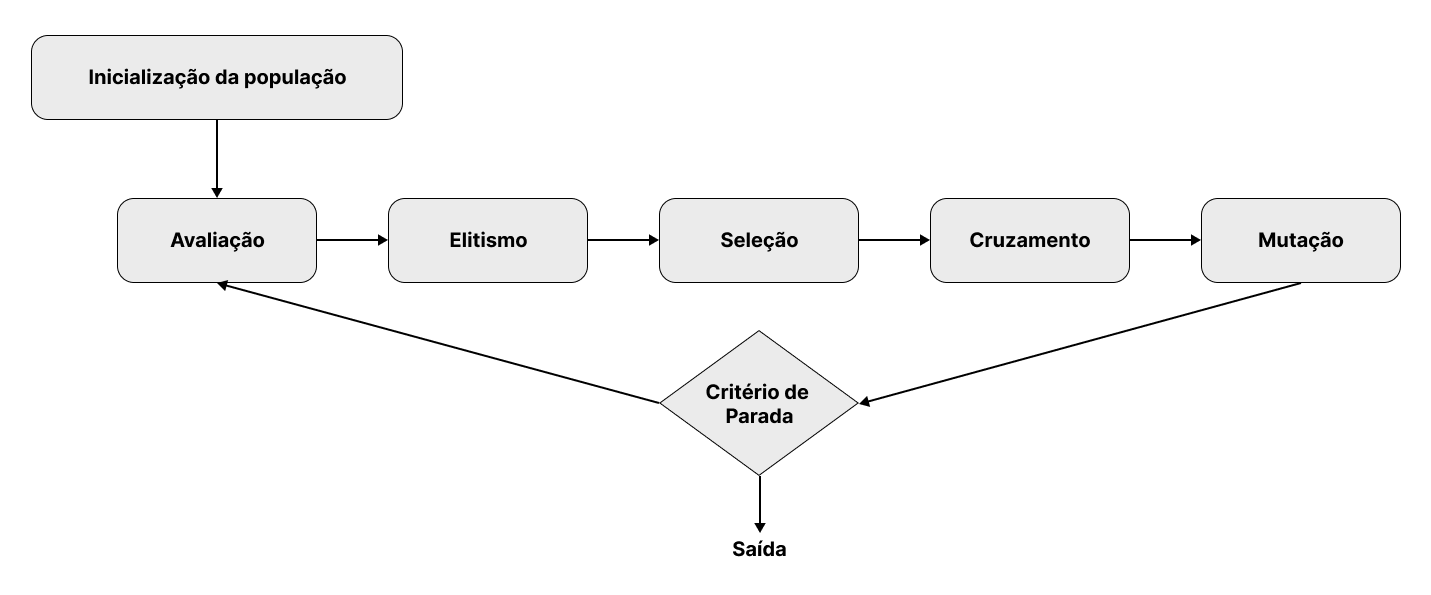
\includegraphics[width=1\textwidth]{figuras/fluxo ag.png}
    \caption*{Fonte: Elaborado pelo autor.}
    \label{fig:fluxo-ag}
\end{figure}

\subsection{Representação dos indivíduos}

Cada indivíduo da população representa uma solução candidata e deve ser codificado de forma adequada ao problema. As representações mais comuns utilizam vetores de inteiros, reais ou binários. A escolha da codificação influencia diretamente o desempenho dos operadores genéticos. Em problemas combinatórios, como o \gls{pcv} \cite{lawler1985traveling}, o Problema de Escalonamento (\textit{scheduling}) \cite{michael1995scheduling} e Problemas de Alocação \cite{burke2004state}, a representação típica é baseada em permutações. Nesses casos, cada indivíduo é codificado como uma sequência que representa uma ordem específica de execução, visita ou alocação de tarefas, elementos ou cidades. Esse tipo de codificação é fundamental para garantir que as soluções geradas sejam válidas. 

Por exemplo, no \gls{pcv}, é necessário que cada cidade seja visitada exatamente uma vez, o que naturalmente leva ao uso de permutações. No entanto, tal escolha impõe desafios adicionais à implementação dos operadores genéticos, especialmente no que diz respeito ao uso de operadores de cruzamento e mutação. Para lidar com essas limitações, foram desenvolvidos \gls{ag}s especializados, conhecidos como \gls{agbo} \cite{syswerda1991schedule}. Esses algoritmos foram projetados especificamente para trabalhar com representações permutacionais, garantindo que os descendentes gerados sejam soluções válidas dentro do espaço combinatório.



\subsection{Inicialização da população}

Essa etapa define o ponto de partida da busca evolutiva e pode afetar a qualidade das soluções encontradas ao longo do processo. A população inicial, composta por $p$ indivíduos (sendo $p$ um parâmetro do algoritmo), pode ser gerada de forma totalmente aleatória ou por meio de estratégias heurísticas que garantam diversidade e viabilidade das soluções. Essas heurísticas utilizam critérios específicos do problema para gerar soluções viáveis com boa qualidade inicial, como menor custo, menor violação de restrições ou melhor balanceamento.

\subsection{Avaliação}

Cada indivíduo é avaliado por meio de uma função de aptidão (\textit{fitness}), que determina a qualidade da solução representada. Essa função pode envolver penalizações por violações de restrições e é essencial para guiar a evolução populacional em direção a soluções melhores.

\subsection{Elitismo}

O elitismo é uma técnica que garante que os melhores indivíduos de uma geração sejam preservados na próxima, evitando perda de boas soluções. Isso é feito copiando um ou mais indivíduos com melhor \textit{fitness} diretamente para a próxima geração, assegurando que a qualidade da população não piore.

\subsection{Seleção}

A seleção define quais indivíduos serão escolhidos para reprodução com base em sua aptidão. Métodos comuns incluem roleta viciada (\textit{roulette wheel}) \cite{goldberg1989genetic}, torneio \cite{miller1995genetic} e seleção ranqueada \cite{goldberg1989genetic}. O objetivo é favorecer indivíduos mais aptos, mantendo certa diversidade genética.

% \textcolor{red}{Mateus, não faz sentido começar a explicar a roleta viciada e não explicar as outras duas técnicas que você citou. É melhor não explicar nenhuma. Seria mais instrutivo para o leitor colocar referências para um livro em que essas técnicas de seleção sejam descritas em detalhe. Para o torneio, vou colocar abaixo alguns links para você pensar se são bons de colocar como referência aqui:}

% \begin{itemize}
% \item \url{https://wpmedia.wolfram.com/sites/13/2018/02/09-3-2.pdf}
% \item \url{https://www.sciencedirect.com/science/article/abs/pii/B9780080506845500082}
% \end{itemize}

% \del{O método da roleta viciada é inspirado em um jogo de roleta em que cada indivíduo recebe uma “fatia” proporcional à sua aptidão. Isso significa que quanto maior a aptidão de um indivíduo, maior a probabilidade dele ser selecionado para reprodução. Esse método, portanto, consiste em calcular a soma total das aptidões da população e, em seguida, atribuir a cada indivíduo uma probabilidade de seleção igual à sua aptidão dividida pela soma total. Em seguida, um número aleatório entre 0 e 1 é gerado, e o indivíduo correspondente à faixa cumulativa onde esse número cai é selecionado. Esse processo é repetido até que o número desejado de indivíduos seja selecionado. Esse método permite que até mesmo indivíduos com menor aptidão tenham alguma chance de serem selecionados, o que contribui para a manutenção da diversidade. No entanto, quando há grandes diferenças entre os valores de aptidão, indivíduos muito fortes podem dominar o processo, levando à perda de diversidade e convergência prematura. Para mitigar esse efeito, podem ser aplicadas técnicas como normalização ou escalonamento da função de \textit{fitness}.}

\subsection{Cruzamento}

O cruzamento é responsável por combinar informações de dois ou mais indivíduos, gerando um ou mais descendentes e é controlada pela \textit{taxa de cruzamento} ($p_c$). Existem diferentes estratégias de cruzamento, e a escolha do método deve considerar a representação dos indivíduos e as características do problema. Em problemas combinatórios com codificação por permutação, o uso de operadores de cruzamento tradicionais pode produzir descendentes inválidos — ou seja, sequências com elementos repetidos ou ausentes. Para contornar essa limitação, foram desenvolvidos os \glspl{agbo}, que utilizam operadores de cruzamento projetados para preservar a ordem relativa ou a posição dos elementos da permutação, garantindo que os descendentes sejam soluções viáveis. Dentre os operadores de cruzamento utilizados nesse contexto, descrevemos a seguir o \textit{Cycle Crossover}, que será um dos operadores de cruzamento aplicado neste trabalho. Uma revisão dos  operadores de cruzamento, incluindo suas características, vantagens e limitações, pode ser encontrada em \citeonline{larranaga}, que analisa comparativamente os principais métodos utilizados no \gls{pcv}. 

O operador \gls{cx} foi projetado para identificar ciclos de posições entre os dois pais e preservar os genes nessas posições do primeiro pai, completando os demais com os genes do segundo. Por exemplo, considere Pai 1: (1 2 3 4 5 6 7 8) e Pai 2: (4 3 2 8 7 6 5 1). O operador começa na primeira posição e percorre os genes dos pais seguindo uma cadeia de referências entre posições equivalentes, até retornar à posição de origem, formando um ciclo. Assim, o ciclo é formado nas posições 0, 3 e 7. Os genes dessas posições são herdados do Pai 1, enquanto os demais (posições 1, 2, 4, 5 e 6) são herdados do Pai 2. O resultado do cruzamento é Filho: (1 3 2 4 7 6 5 8). A Figura~\ref{fig:cx-exemplo} ilustra o funcionamento do \gls{cx}, destacando os ciclos encontrados e os genes herdados de cada pai. Para garantir diversidade genética e simetria, o \gls{cx} pode gerar um segundo filho, onde a lógica é invertida, os genes do ciclo são herdados do Pai 2, e os demais do Pai 1.

\begin{figure}[!htb]
    \centering
    \caption{Exemplo do operador \textit{Cycle Crossover}.}
    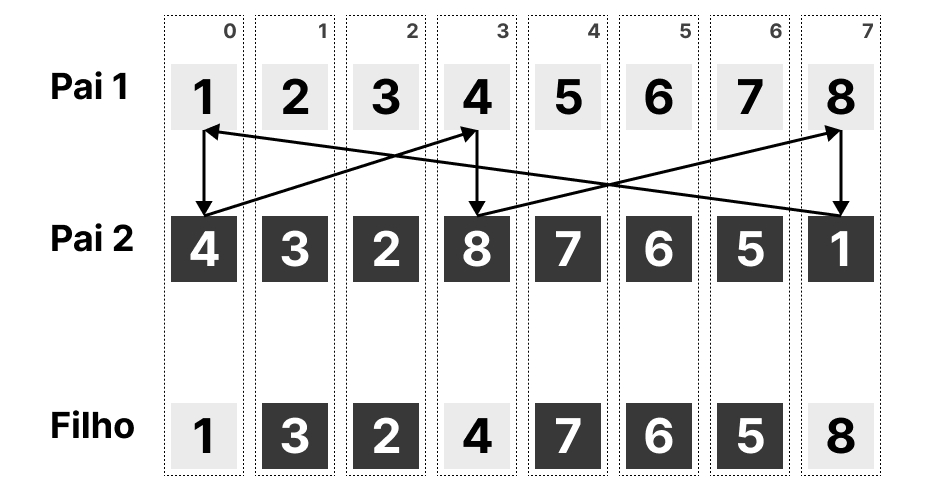
\includegraphics[width=0.7\textwidth]{figuras/cycle crossover.png}
    \caption*{Fonte: Elaborado pelo autor.}
    \label{fig:cx-exemplo}
\end{figure}

% \del{O funcionamento do operador \gls{ox} constrói os filhos escolhendo um segmento de um dos pais e preservando a ordem relativa dos genes do outro pai. Por exemplo, considere Pai 1: (1 2 3 4 5 6 7 8) e Pai 2: (2 4 6 8 7 5 3 1). Supondo que o segmento selecionado vá da posição 2 à 4, os filhos iniciam com esse trecho copiado diretamente: (X X \textbf{3 4 5} X X X) e (X X \textbf{6 8 7} X X X). Os genes restantes são preenchidos na ordem em que aparece no outro pai, a partir do fim do seguimento, omitindo-se os genes que já estão presentes no filho. Quando o final sequência é alcançada, continua-se a partir da primeira posição, resultando em Filho 1: (8 7 \textbf{3 4 5} 1 2 6) e Filho 2: (4 5 \textbf{6 8 7} 1 2 3).}

Já o \gls{pmx} é um operador que preserva tanto a posição quanto os valores de um segmento selecionado entre os pais. Ele funciona estabelecendo um mapeamento entre os genes presentes no segmento selecionado aleatoriamente dos dois pais e utilizando esse mapeamento para preencher os genes restantes nos dois filhos gerados, garantindo a viabilidade das permutações. Por exemplo, considere Pai 1: (1 2 3 \textbf{4 5 6} 7 8), Pai 2: (3 7 5 \textbf{1 6 8} 2 4) e
Segmento: posições 3 ao 5. As subsequências de mapeamento são [4 5 6] e [1 6 8], definindo os mapeamentos $4\leftrightarrow1$, $5\leftrightarrow6$ e $6\leftrightarrow8$. Essas subsequências são trocadas e copiadas diretamente para os filhos nas mesmas posições. Os demais elementos são preenchidos com base na sequência do outro pai, corrigidos com os mapeamentos quando necessário. Resultando em Filho 1: (4 2 3 \textbf{1 6 8} 7 5) e Filho 2: (3 7 8 \textbf{4 5 6} 2 1).

\subsection{Mutação}

O operador de mutação introduz pequenas alterações aleatórias nos descendentes gerados após o cruzamento, com o objetivo de preservar a diversidade genética e evitar estagnação prematura. O operador de mutação pode modificar um ou mais genes de um indivíduo, e sua aplicação é controlada por uma \textit{taxa de mutação}  ($p_m$) definida pelo usuário. Em \glspl{ag} tradicionais com representações binárias ou de inteiros, a mutação pode ser realizada por inversão de bits ou por pequenas perturbações nos valores dos genes. No entanto, em problemas combinatórios com codificação por permutação — como os abordados pelos \glspl{agbo} —, operadores de mutação convencionais podem gerar soluções inválidas, violando a restrição de que cada elemento deve aparecer exatamente uma vez na sequência. Para contornar esse problema, os \glspl{agbo} utilizam operadores de mutação especialmente desenhados para atuar sobre permutações, mantendo a viabilidade das soluções. \citeonline{larranaga} apresenta de forma detalhada dos principais operadores de mutação aplicáveis a representações permutacionais.


% \textcolor{green!50!black}{Mateus, seguindo a mesma linha do crossover, acho melhor não entrar em detalhes aqui. O momento de explicar quais operadores foram usados é lá nos resultados preliminares. Explique lá cada operador que você usou no seu algoritmo!}

% \del{O operador \gls{dm} consiste em selecionar aleatoriamente um segmento contínuo da permutação e deslocá-lo para outra posição dentro do indivíduo. Os elementos do segmento são removidos de sua posição original e inseridos na nova posição, enquanto os demais genes são realocados de forma a manter a ordem relativa e a viabilidade da permutação. O operador \gls{em} realiza a troca direta de posição entre dois genes escolhidos aleatoriamente dentro do indivíduo. Já o \gls{ivm} seleciona aleatoriamente um segmento contínuo, remove-o da permutação e o insere em uma posição aleatória invertendo a ordem dos elementos contidos nesse intervalo. O operador \gls{sm} seleciona um segmento contínuo da permutação e embaralha aleatoriamente os elementos dentro desse intervalo. O operador \gls{ism} consiste em remover um gene de sua posição original na permutação e inseri-lo em outra posição aleatória do indivíduo. Os demais genes são deslocados de forma a manter a integridade da sequência. Por último, o operador \gls{sim} seleciona aleatoriamente dois pontos de corte na permutação, e o segmento entre eles é invertido.}

\subsection{Critério de Parada}

O algoritmo genético pode ser interrompido com base em diferentes critérios: número máximo de gerações, tempo de execução, ausência de melhoria nas soluções ou convergência da população. A escolha adequada desse critério é fundamental para equilibrar custo computacional e qualidade das soluções obtidas.

\subsection{Aspectos Estocásticos e Reprodutibilidade}

Uma característica fundamental dos algoritmos genéticos é sua dependência de mecanismos estocásticos. Isso significa que suas execuções envolvem fatores aleatórios, como a seleção de pais, aplicação de mutações e amostragem inicial, tornando os resultados dificilmente reprodutíveis. No entanto, essa aleatoriedade também confere aos AGs uma capacidade robusta de escapar de ótimos locais e encontrar boas soluções em espaços de busca complexos.

Para garantir reprodutibilidade parcial em experimentos científicos, é comum a fixação de uma semente (\textit{seed}) para os geradores de números aleatórios utilizados. Mesmo assim, pequenas variações podem surgir em função de paralelismo ou diferenças na arquitetura de hardware, o que reforça a necessidade de realizar múltiplas execuções e reportar medidas estatísticas sobre os resultados.

\section{Algoritmos Genéticos de Chaves Aleatórias Enviesadas}

\citeonline{bean1994genetic} introduziu os \gls{agca}, uma entre diversas variações dos \glspl{ag}, para problemas de sequenciamento. Nessa classe de algoritmos genéticos, os cromossomos são vetores de números reais aleatórios no intervalo $[0,1]$. Um decodificador determinístico interpreta cada vetor e o transforma em uma solução viável para o problema, permitindo assim a avaliação de sua aptidão. O algoritmo é elitista (a população é dividida em dois conjuntos: Elite e Não-Elite) e a cada geração são introduzidos mutantes. Para gerar uma nova população, o \gls{agca} utiliza o cruzamento entre pares de indivíduos selecionados aleatoriamente de toda a população. 

No entanto, a seleção desses pares pode seguir estratégias diferentes. No \gls{agcae} \cite{ericsson2002genetic, gonccalves2002hybrid, gonccalves2011biased, gonccalves2004evolutionary}, um dos pais é sempre escolhido da elite, composta pelos $p_e$ melhores indivíduos da população $p$, enquanto o outro é selecionado do grupo não-elite, formado pelos $p - p_e$ indivíduos restantes, sendo $p_e < p - p_e$, conforme ilustrado na Figura~\ref{fig:funcionamento-brkga}. Isso aumenta a probabilidade de que boas características genéticas sejam passadas adiante. Outro fator que contribui com a propagação de boas características é o \textit{cruzamento uniforme parametrizado}, operador utilizado no \gls{agcae}. Nesse operador, cada gene tem uma probabilidade $\rho_e > 0.5$ (definida pelo usuário) de herdar o alelo do pai de elite. Para um cromossomo com $n$ genes, o $i$-ésimo gene tem a probabilidade de $\rho_e$ de assumir o valor do $i$-ésimo gene do pai de elite e $1 - \rho_e$ de assumir o valor do $i$-ésimo gene do pai de não-elite. Esse mecanismo de cruzamento, aliado à seleção enviesada e à introdução de mutantes a cada geração, confere ao \gls{agcae} uma capacidade robusta de convergência para regiões promissoras do espaço de busca, equilibrando exploração e intensificação.

\begin{figure}[!htb]
    \centering
    \caption{Esquema ilustrativo do funcionamento de um AGCAE.}
    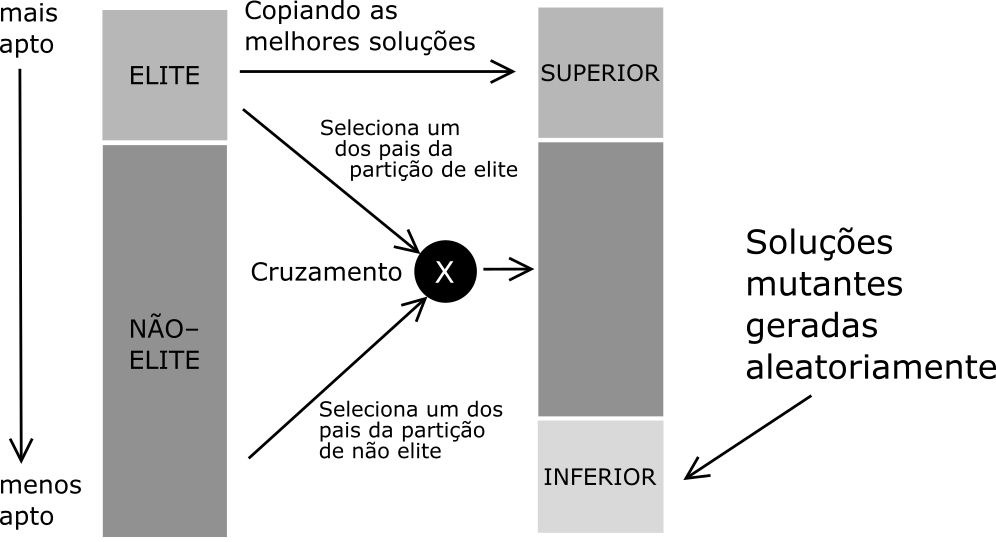
\includegraphics[width=0.7\textwidth]{figuras/funcionamento agcae.png}
    \label{fig:funcionamento-brkga}
    \caption*{Fonte: Adaptado de \citeonline{gonccalves2011biased}.}
\end{figure}

Um dos principais benefícios dos \glspl{agca}, especialmente em sua versão enviesada, é a separação conceitual entre os componentes dependentes e independentes do problema. O operador genético e os mecanismos de seleção atuam sobre uma representação genérica baseada em chaves aleatórias, ou seja, sobre vetores de números reais no intervalo $[0,1]$. Essa parte do algoritmo é independente do problema, podendo ser reutilizada em diferentes contextos sem modificações. Por outro lado, a decodificação e a avaliação da aptidão são partes específicas do problema. O decodificador é responsável por transformar um vetor de chaves em uma solução viável para o problema-alvo, respeitando suas restrições e características estruturais. Essa transformação depende fortemente do domínio de aplicação e deve ser cuidadosamente projetada para garantir que pequenas variações nos cromossomos gerem soluções correspondentes com diferenças proporcionais de qualidade.